A cone frustum has base radius $b$, top radius $a$, and height $h$, as shown in Fig.~1.8. Assuming that one of the following quantities is the volume of the frustum, which one is it? (Don't solve the problem from scratch, just check special cases.)

$$\frac{\pi h}{3}(a^2 + b^2),\quad \frac{\pi h}{2}(a^2 + b^2),\quad \frac{\pi h}{3}(a^2 + ab + b^2),$$
$$\frac{\pi h}{3} \cdot \frac{a^4 + b^4}{a^2 + b^2},\quad \pi hab.$$

\begin{center}
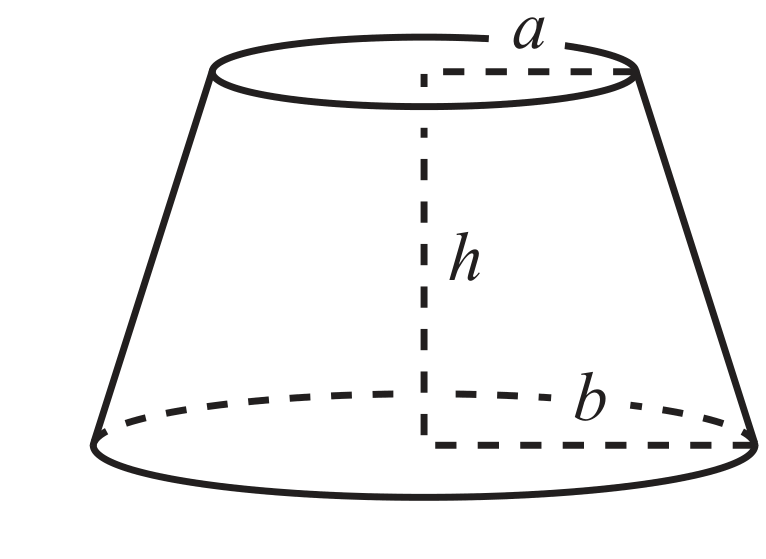
\includegraphics[width=0.45\linewidth]{figures/qfig1.png} \\
Fig.~1.8
\end{center}